
%title page
\begin{frame}
\titlepage
\end{frame}

\section{Introduction}

\begin{frame}{Big data in astroparticle physics (APP)}
%или "Астрофизика - современное состояние"))
\small
\vspace{-2em}
\begin{columns}
  \begin{column}[t]{0.55\textwidth}
    \begin{center}
     \vspace{-1em}
%       \includegraphics[width=1.5\textwidth]{pics/appec_base4.pdf}
      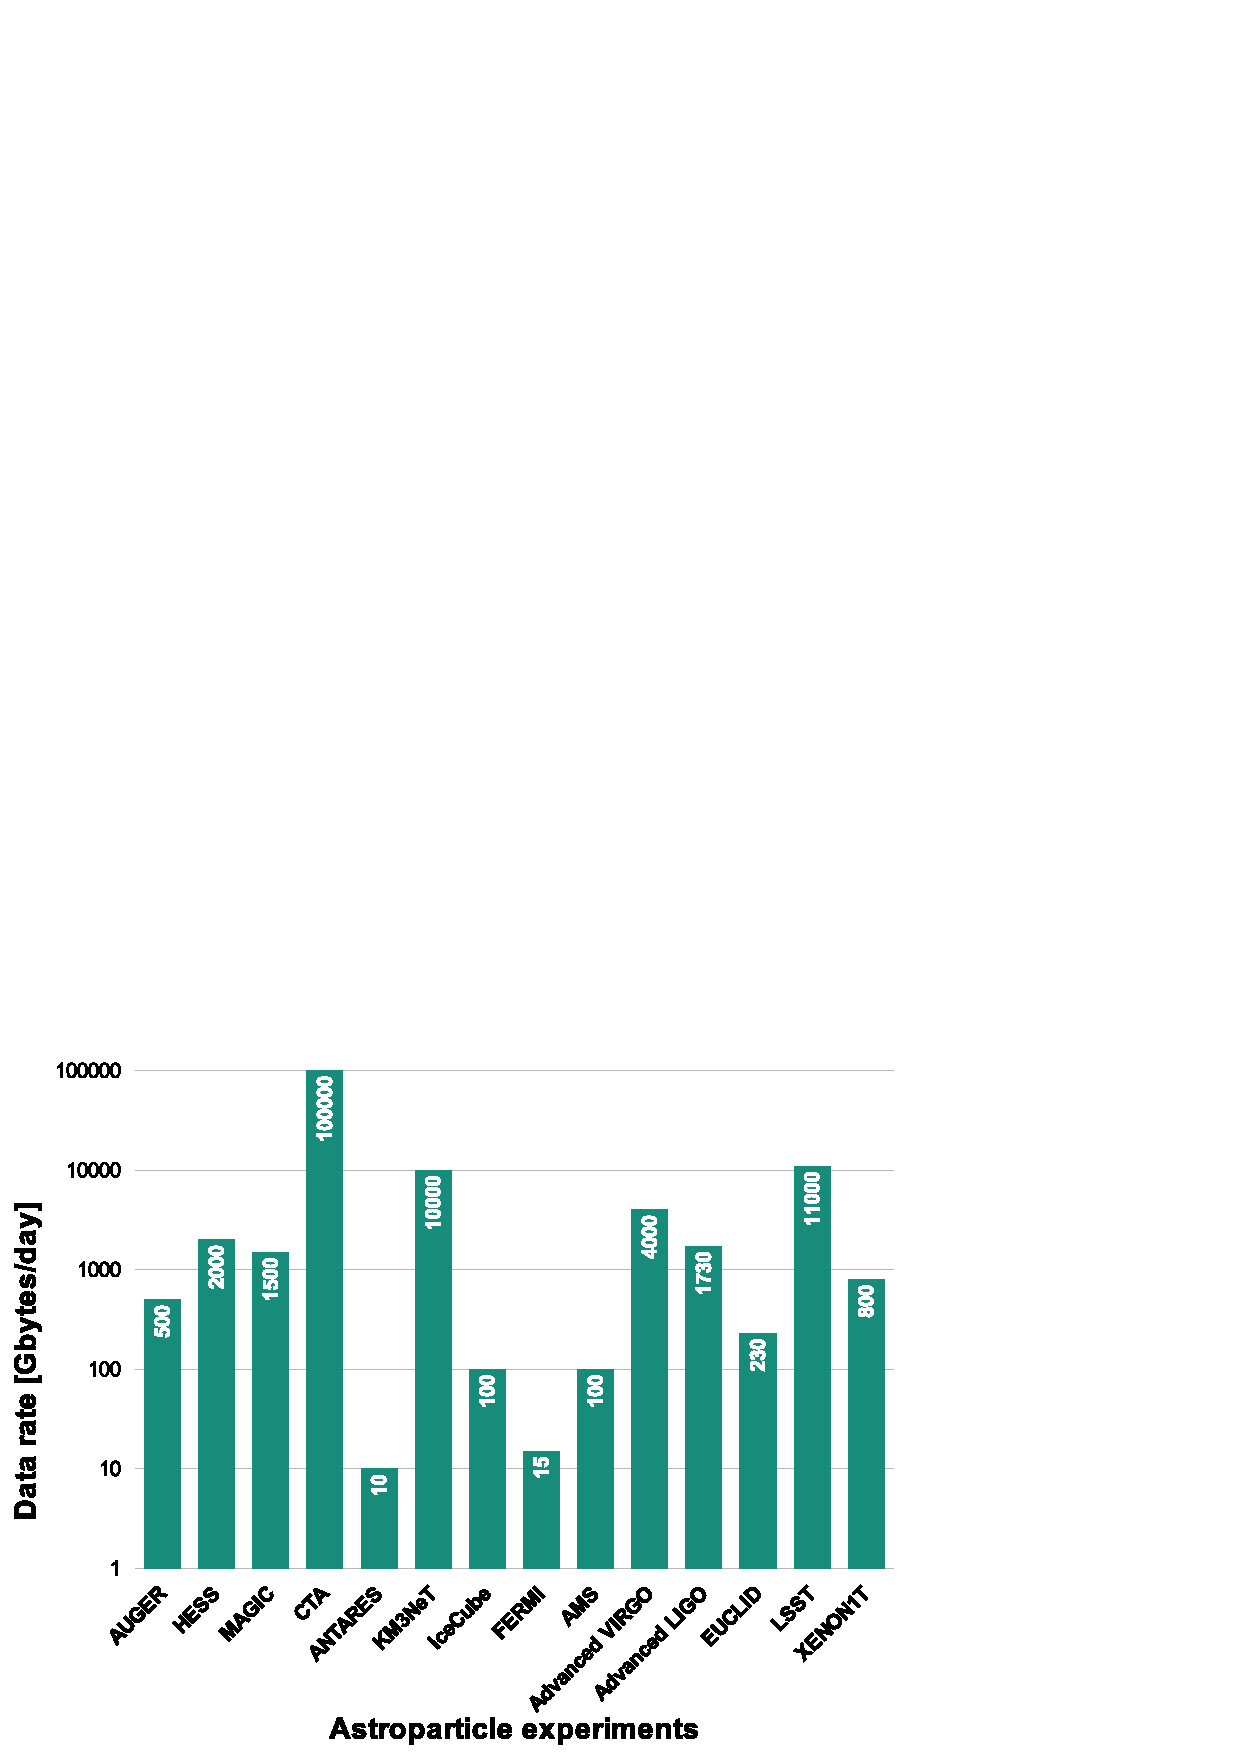
\includegraphics[width=1.12\textwidth]{pics/appec_computing-diagram.pdf}
    \end{center}
    \vspace{-2\parsep}
    \small Modern astroparticle experiments data rate [Gbytes/day]\footnotemark[1] %, source: APPEC brochure on Computing, 2016}
  \end{column}
  \hfill
  \begin{column}[t]{0.42\textwidth}
    \begin{itemize}
    \item Wide range of experiments;
    \item More than hundred years of cosmic particle measurements;
    \item Looking at the same sky with different detectors;
    \item Common data rate for astropartical physics experiments all together is a few PBytes/yeary, which is comparable to the current LHC output\footnotemark[1] % \textcolor{red}{(ссылка на брощюру!!!)}
    \item Big data for deep learning
    \end{itemize}

%     \textcolor{red}{TODO: дописать текста, чтобы сбалансирвоать дизайн страницы}
  \end{column}
\end{columns}
  \footnotesize\footnotetext[1]{Berghöfer T., Agrafioti I. et all. Towards a model for computing in European astroparticle physics, Astroparticle Physics European Coordination committee, 2016\\~}
%   \\http://www.appec.org/wp-content/uploads/Documents/Docs-from-old-site/AModelForComputing-2.pdf}
\end{frame}

\begin{frame}{Software data life cycles}% and information management
\begin{itemize}
\item \textbf{Data Life Cyce (DLC)} is ...
\item \textbf{Data engineers} are ...
\end{itemize}

\vspace{-1ex}
\centering
\includegraphics[width=0.65\textwidth]{pics/data_lifecycle_illust.jpg}
\end{frame}

\begin{frame}{Data engineering in APP}

\begin{columns}
    \begin{column}[t]{5cm}
        \begin{itemize}
        \item  Introduction \textcolor{kit-green100}{$\rightarrow$ we are here}
        \item  GRADLC initiative and main objectives
        \item  DCL in APP - specific
        \item  DCL architecture
        \item  Experiments and data specific
        \item  Joint analysis scheme
        \item  Possible solutions
        \item  Outlook and future work
        \end{itemize}
    \end{column}

    \begin{column}[t]{5cm}
%         \includegraphics[width=0.65\textwidth]{pics/DE_fun.jpeg}
    paste a croped picture here
    \end{column}
    \end{columns}
\end{frame}

\begin{frame}{German-Russian Astroparticle \\Data Life Cycle Initiative\footnotemark[1]}
\vspace{-1.4em}
% \textcolor{red!50!black}{Change the collboration picture}
\begin{center}
  \includegraphics[width=0.9\textwidth]{pics/Collab-3.pdf}
\end{center}
\footnotesize\footnotetext[1]{Granted by RSF-Helmholtz Joint Research Groups}
\end{frame}

% \begin{frame}{KASCADE-Grande}
% \begin{itemize}
%   \item Proposed in 1989---disassembled in 2013;
%   \item Aimed at studying
%   high-evergy (galactic) cosmic rays by observing extensive air showers (EAS);
% %   processes at the edge of the Galaxy and beyond by observing extended atmospheric showers (EAS);
%   \item Consisted of:
%   \begin{itemize}
%     \item scintillators detecting $e$, $\gamma$, $\mu$:
%     \begin{itemize}
%   %сцинтиляторы, различают e, gamma, mu
%     \item KASCADE---256 stations;
%     \item GRANDE---37 stations;
%     \end{itemize}
%  %один большой калориметр
%     \item Hadronic callorimeter;
%  %радиодетектор
%     \item Digital radio array LOPES detecting $e$, $e^{+}$;
% % позволяющих наблюдать различные компоненты ливня
%   \end{itemize}
%   \item Important features of cosmic-ray spectrum have been obtained. The data analysis is ongoing;
% %  благодаря данным с эксперимента было открыто много всего ополезного, при этом анлиз данных продолжается. новые статьи выходят
%   \item KCDC (\textbf{K}ASCADE \textbf{C}osmic Ray \textbf{D}ata \textbf{C}enter, \textcolor{blue}{\texttt{http://kcdc.ikp.kit.edu}}) is a dedicated portal where all the data collected are available online. % At the moment
% %   к настоящему времени все данные эксперимента опубликованы и доступны онлайн, для этих целей был сделан
% %  принциально принципиально новый и крутой на тот момент портал KCDC
% % \textcolor{red!50!black}{Add the kcdc logo in the center of the slide}
% \end{itemize}
%
% \begin{tikzpicture}[remember picture,overlay]
%   \node[xshift=-12ex,yshift=-21ex] at (current page.north east){%
%     \includegraphics[width=0.3\textwidth]{pics/KCDC-Logo.png}
%   };
% \end{tikzpicture}
% % \parbox[t][0pt]{0pt}{
% %   \vspace{-0.63\textheight}
% %   ~\hspace{0.68\textwidth}\includegraphics[width=0.3\textwidth]{pics/KCDC-Logo.png}
% % }
% \end{frame}
%
%
%
% \begin{frame}{TAIGA}
% \footnotesize
% \vspace{-1em}
% \begin{itemize}
%  \item Started in the mid 90s, is still operating and continiously enhancend
% %  \item Currently consists of 4 detectors presented + TUNKA IACT is under construction;
% \end{itemize}
% \vspace{-2em}
% \begin{minipage}[t]{0.31\textwidth}
%   \begin{block}{\small Tunka-133}
%     \parbox[c][0.20\textheight][t]{1\textwidth}{
%       \centering
%       \includegraphics[width=0.7742\textwidth]{pics/Tunka-133.jpg}
%     }
%     \hfill
%     \parbox[c][0.15\textheight][t]{1\textwidth}{
%       \begin{itemize}
%         \setlength{\itemsep}{0pt}
%         \item 133 photomultipliers
%         \item measures EAS Cherenkov light
%       \end{itemize}
%     }
%   \end{block}
% \end{minipage}
% \hfill
% \begin{minipage}[t]{0.31\textwidth}
%   \begin{block}{\small Tunka-Rex}
%     \parbox[c][0.20\textheight][t]{1\textwidth}{
%       \centering
%       \includegraphics[width=0.7742\textwidth]{pics/Tunka-Rex.jpg}
%     }
%     \\
%     \parbox[c][0.15\textheight][t]{1\textwidth}{
%       \begin{itemize}
%         \setlength{\itemsep}{0pt}
%         \item 63 antennas
%         \item measures EAS radio-emission
%       \end{itemize}
%     }
%   \end{block}
% \end{minipage}
% \hfill
% \begin{minipage}[t]{0.31\textwidth}
%   \begin{block}{\small Tunka-HiSCORE}
%     \parbox[c][0.20\textheight][t]{1\textwidth}{
%       \centering
%       \includegraphics[width=0.7742\textwidth]{pics/Tunka-HiSCORE.jpg}
%     }
%     \\
%     \parbox[c][0.15\textheight][t]{1.1\textwidth}{
%       \begin{itemize}
%         \setlength{\itemsep}{0pt}
%         \item 47$\times$4 photomultipliers
%         \item measures EAS Cherenkov light
%       \end{itemize}
%     }
%   \end{block}
% \end{minipage}
%
% \vspace{-1ex}
% \begin{minipage}[t]{0.48\textwidth}
%   \begin{block}{\small Tunka-Grande}
%     \parbox[c][0.21\textheight][t]{0.43\textwidth}{
%       \includegraphics[width=0.50\textwidth]{pics/Hiller_Roman-005.jpg}
%     }
%     \hfill
%     \parbox[c][0.21\textheight][t]{0.55\textwidth}{
%       \begin{itemize}
%         \setlength{\itemsep}{0pt}
%         \item 380 scintillators 0.64m$^2$ each
%         \item measures $e$/$\mu$ from EAS
%       \end{itemize}
%     }
%   \end{block}
% \end{minipage}
% \hfill
% \begin{minipage}[t]{0.48\textwidth}
%   \begin{block}{\small Tunka-IACT}
%     \parbox[c][0.21\textheight][t]{0.43\textwidth}{
%       \includegraphics[width=0.50\textwidth]{pics/Tunka-Iact.jpg}
%     }
%     \hfill
%     \parbox[c][0.21\textheight][t]{0.55\textwidth}{
%       \begin{itemize}
%         \setlength{\itemsep}{0pt}
%         \item Imaging Air Cherenkov Telescopes
%         \item is being extended
%       \end{itemize}
%     }
%   \end{block}
% \end{minipage}
% \end{frame}
%
